% -----------------------------------------------------------------------
% --- DOCUMENT ---
% -----------------------------------------------------------------------
\documentclass[11pt, a4paper, french, twoside]{article}

% -----------------------------------------------------------------------
% --- PACKAGE ---
% -----------------------------------------------------------------------
\usepackage[french]{babel}

% Font
\usepackage[utf8]{inputenc}
\usepackage[T1]{fontenc}

% Marge du document
\usepackage[top=3.5cm,
	bottom=3cm,
	left=2cm,
	right=2cm,
	footskip=1.5cm,
	headheight=1.5cm,
	headsep=0.9cm]{geometry}

% Gérer les positionnement d'images
\usepackage{float}

% Import de fichier externe
\usepackage{graphicx}

% Mise en forme des URL
\usepackage{url}

% Informations sur un document compilé en PDF et les liens externes / internes
\usepackage{hyperref}

% Pour les entêtes
\usepackage{fancyhdr}

% -----------------------------------------------------------------------
% --- INFORMATION SUR LE DOCUMENT
% -----------------------------------------------------------------------

% Information sur le document
\hypersetup{
	pdfauthor = {Kirushnapillai Sathiya, Monteverde Mathieu, Zucca Michela},                    % Auteurs
	pdftitle = {Project Cours Scala},                         % Titre du document
	pdfsubject = {Description du projet},                % Sujet
	pdfstartview={FitH}}                            % ajuste la page à la largueur de l'écran

% -----------------------------------------------------------------------
% --- EN-TETE ET PIED DE PAGE ---
% -----------------------------------------------------------------------
\pagestyle{fancy}
\fancyhf{} % Supprime les entetes et pieds de page existants

\fancyhead[LE,RO]{Description du projet\\}
\fancyhead[LO]{
\includegraphics[width=4cm]{images/logo_heig.png}}
\fancyfoot[LE,RO]{\thepage{}}
\fancyfoot[RE]{Kirushnapillai Sathiya, Monteverde Mathieu, Zucca Michela}
\fancyfoot[LO]{Project Cours Scala}
\renewcommand{\footrulewidth}{1pt}


\title{Project Cours Scala \\ Description du projet}
\author{Kirushnapillai Sathiya, Monteverde Mathieu, Zucca Michela}
\date{2018}


\begin{document}
	\selectlanguage{french}
	\graphicspath{ {images/} }
	
	% Espacement entre les lignes
	\newcommand{\HRule}{\rule{\linewidth}{0.5mm}}
	
	% Page de garde
	\begin{titlepage}
    \begin{center}

	 \vspace{0.5cm}
     {\fontsize{1.5cm}{1.8cm} \bf Project Cours Scala}\par
     \vspace{0.5cm}
     {\fontsize{0.9cm}{1.3cm} \selectfont Description du projet}\par
     \vspace{3cm}
     \vfill
        
        % Author and supervisor
        \begin{minipage}{0.4\textwidth}
        	\begin{flushleft} \large
        		\textbf{Auteurs:}\\
        		\textsc{Kirushnapillai} Sathiya \\
        		\textsc{Monteverde} Mathieu \\
        		\textsc{Zucca} Michela
        	\end{flushleft}
        \end{minipage}
        \begin{minipage}{0.4\textwidth}
            \begin{flushright} \large
                \textbf{Professeur:} \\
                \textsc{Fatemi} Nastaran \\
            \end{flushright}
        \end{minipage}
    
        \vfill
    \begin{minipage}{0.4\textwidth}
    	\begin{flushleft} \large
       		
\includegraphics[width=5cm]{images/logo_heig.png}
        \end{flushleft}

	\end{minipage}
	\begin{minipage}{0.4\textwidth}
	    \begin{flushright}
			
\includegraphics[width=5cm]{images/logo-hes-so.jpg}
		\end{flushright}
	\end{minipage}


        % Bottom of the page
        \today
        
    \end{center}
\end{titlepage}

	
	% Recommencer la numérotation des pages à "1"
	\setcounter{page}{1}
	\newpage
	
	% Espacement des paragraphes
	\setlength{\parskip}{0.2cm}
	
	\section{Contexte}
	\label{sec:contexte}
		Ce projet s'effectue dans le cadre du cours SCALA 2018. L'objectif est de réaliser une application Web en utilisant la technologie Scala Play pour le back-end et Slick pour la base de données. Le choix de la technologie front-end est libre.
		
	\section{Description}
	\label{sec:description}
	
		\subsection{Buts}
		\label{subsec:buts}
		L'idée de ce projet est de proposer une plateforme Web permettant de partager des événements avec ses utilisateurs. Un utilisateur inscrit au préalable (subsequenceset faisant partie d'une organisation) pourra enregistrer des événements (par exemple un concert, une journée portes-ouvertes, un festival, etc.) en spécifiant des informations comme par exemple la localisation (coordonnées GPS ou adresse), une description, une ou plusieurs dates et des horaires.
		
		Un visiteur du site pourra ensuite rechercher les événements situés dans une certaines zone (par exemple dans un rayon de 10km autour de Lausanne) en spécifiant différents paramètres comme la date ou l'heure. 
		
		Le but est d'offrir un service indépendant de tout réseau social permettant à ses utilisateurs de trouver facilement des événements culturels ou festifs autour d'eux. 
		
		Une organisation est une entité (entreprise, commune, association, etc.) qui peut-être certifiée. Cela permet un certain contrôle sur le type d'événements qui sont créées (éviter les faux événements, les fêtes d'anniversaire, etc.).
	
	\section{Fonctionnalités}
	\label{sec:fonctionnalites}
		Cette section liste les fonctionnalités qu'offrira la plateforme pour les différents acteurs. 
		
		\subsection{Visiteurs}
		\label{subsec:visiteurs}
			Un utilisateur non-authentifié de l'application Web pourra: 
			
			\begin{itemize}
				\item Voir une liste d'événements
				\item Filtrer une liste d'événements par data
					\begin{itemize}
						\item Choisir une date exacte
						\item Choisir une plage avec date de début et date de fin
					\end{itemize}
				\item Filtrer une liste d'événements par lieu géographique
					\begin{itemize}
						\item Choisir une ville départ
						\item Choisir un rayon de recherche autour de cette ville
					\end{itemize}
				\item Rechercher un événement
					\begin{itemize}
						\item Recherche par nom d'événement
						\item Recherche par organisation
					\end{itemize}
				\item Filtrer une liste d'événement par thème
				\item Voir le détail d'un événement
				\item Créer un compte sur la plateforme
					\begin{itemize}
						\item E-mail
						\item Mot de passe
						\item Nom d'utilisateur
						\item Prénom
						\item Nom de famille
					\end{itemize}
			\end{itemize}
		
		\subsection{Utilisateur inscrit}
		\label{subsec:utilisateur_inscrit}
			Un utilisateur authentifié pourra:
			
			\begin{itemize}
				\item Afficher son profil
				\item Modifier les informations de son profil
				\item Supprimer son profil
				\item Créer une organisation
					\begin{itemize}
						\item Spécifer le type d'organisation (Entrprise, association, ville, etc.)
						\item Spécifier le nom de l'organisation
						\item Spécifier l'adresse
						\item D'autres informations si nécessaire
					\end{itemize}
				\item Afficher les informations des organisations dont il fait partie
				\item Ajouter des utilisateurs à une organisation
				\item Modifier les informations des organisations dont il fait partie
				\item Supprimer une organisation
				\item Créer un événement au nom d'une organisation dont il fait partie
					\begin{itemize}
						\item Titre
						\item Description
						\item Prix
						\item Lieu (Adresse ou coordonées géographiques)
						\item Date de début
						\item Date de fin
						\item Horaires
						\item Organisation
						\item Thèmes de l'événement
					\end{itemize}
				\item Modifier un événement d'une organisation dont il fait partie
				\item Supprimer un événement d'une organisation dont il fait partie
			\end{itemize}
		
	\section{Structure}
	\label{sec:structure}
		La figure \ref{fig:er} illustre le schéma entité-relation de la base de données du projet. L'application comporte des utilisateurs (User), des organisations (Organization) et des évenements (Event). Pour chaque entité, les opérations de base (CRUD) seront fournies : Afficher, créer, modifier et supprimer. Cependant, seuls les utilisateurs liés à une organisation peuvent créer, modifier et supprimer des événements.
		
		Pour cette première ébauche, chaque événement possède un ou plusieurs thèmes (Theme) qui permettront aux visiteurs de filtrer leurs recherches. Les thèmes permettent également aux utilisateurs inscrits d'être notifié d'un nouvel événement selon leurs préférences (Ce dernier point est pour l'instant optionnel).
		
		Et enfin, l'application permettra également aux utilisateurs inscrits de commenter un événement.
		
		\begin{figure}[h]
			\centering
			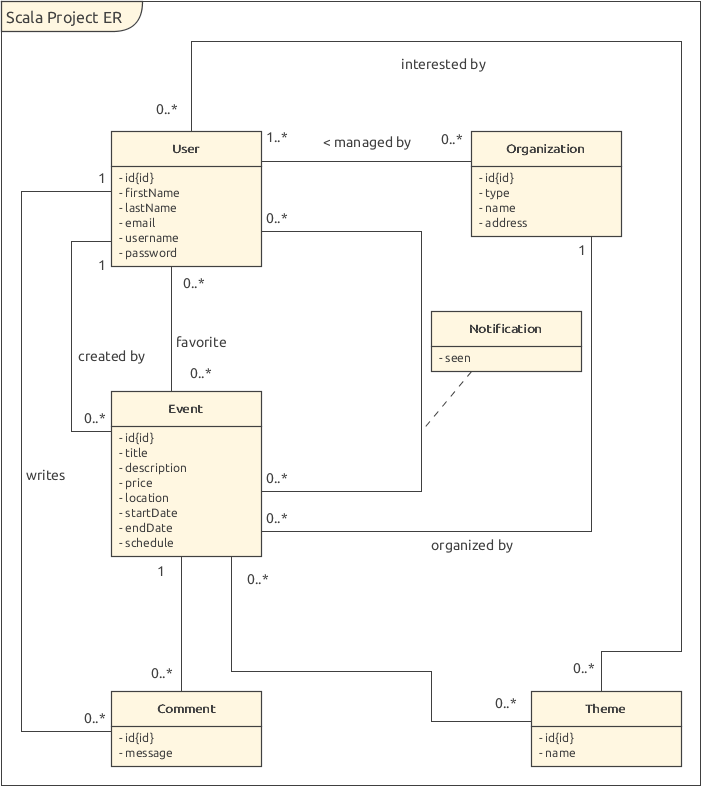
\includegraphics[width=0.8\linewidth]{images/project_ER.png}
			\caption{Schéma entité-relation de la base de données}
			\label{fig:er}
		\end{figure}
	
\end{document}
